\documentclass{article}

\usepackage{graphicx}
\usepackage{natbib}
\usepackage{amsmath}
\usepackage{hyperref}

\newcommand{\urlGammaCat}{\url{https://github.com/gammapy/gamma-cat}}

\title{GPS sky model for CTA 1DC}

\author{
  Zanin, Roberta
  \and
  Deil, Christoph
  \and
  Christofari, Pierre
}

%\date{\today} % Date for the report

\begin{document}

\maketitle

\begin{center}
\begin{tabular}{lr}
Status: & Work in progress \\
Version: & \date{\today} \\
Repository: & \url{https://github.com/gammasky/cta-dc} \\
\end{tabular}
\end{center}

\begin{abstract}
Abstract text
\end{abstract}

\section{Introduction}

What is this?

TODO: for which datasets was this model used? GPS, GC, EGAL?

\section{Sky model components}

\subsection{Known bright sources}

\subsubsection{gamma-cat}

We use gamma-cat (\urlGammaCat) for most known VHE sources,
except the ones listed in sections TODO and table TODO.

\subsubsection{Image sources}

See sky\_model/image\_sources

\subsubsection{Binaries}

See \verb=sky_model/binaries= and Table~\ref{tab:binaries}.

\begin{table*}[t]
\caption{
%
Gamma-ray binaries.
%
}
\label{tab:binaries}
\centering
\begin{tabular}{lrr}
\hline
Source Name  & GLON & GLAT \\
             & deg & deg \\
\hline
LS 5039      & 16.902 & -1.278 \\
PSR B1259-63 & 304.186 & -0.987 \\
\hline
\end{tabular}
\end{table*}

\subsection{Synthetic populations of faint sources}

\subsubsection{Pulsar wind nebulae}

\subsubsection{Supernova remnants}

\subsubsection{Composites}

\subsection{Diffuse emission}

TODO: need short description of ISO and GAL diffuse emission components, no?

\section{Illustrations and Checks}

\subsection{Spatial distribution in the Galaxy}

Show and discuss X, Y, Z, distance distribution of sources in the Galaxy.

\subsection{Spatial distribution on the Sky}

Show and discuss GLON, GLAT distribution

\subsection{Source sizes}

Do physical and observed size together here should be OK?

\subsection{Source fluxes}

Look at one or more integral flux measures.

Discuss CTA sensitivity and which sources might be visible here or later?

\subsection{Source spectra}

Just as an example: For PWN spectra, see Fig.~\ref{fig:pwn_spec}

\begin{figure}[t]
\begin{center}
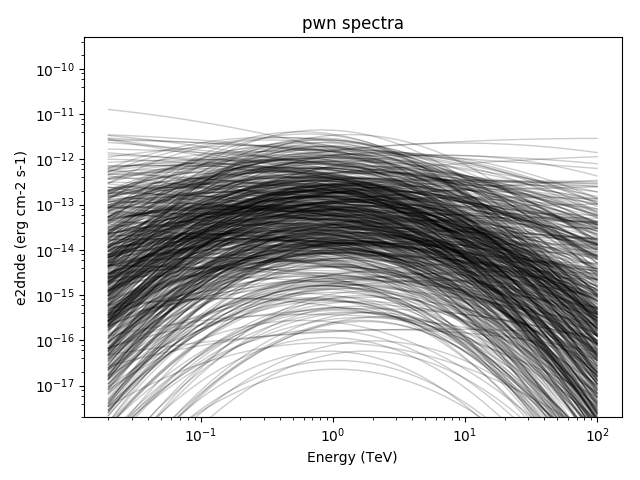
\includegraphics[width=1.0\textwidth]
{../sky_model_checks/ctadc_skymodel_gps_sources_spectra_pwn}
\caption{PWN spectra (just as an example of a Figure)}
\label{fig:pwn_spec}
\end{center}
\end{figure}


How do we compare to HGPS \citep{2013arXiv1307.4868C}?

\section{Conclusions}

How did we do? What can be done better in DC2?


\bibliographystyle{apalike}

\bibliography{cta_1dc_gps_sky_model}

\end{document}
